\documentclass[12pt]{report}

\usepackage[default]{sourcesanspro}
\usepackage[T1]{fontenc}
\usepackage{titlesec}
\usepackage{xcolor}
\usepackage{graphicx}
\usepackage{fancyhdr}
\usepackage{everypage}
\usepackage{soul} % For letter spacing and background color
\usepackage[letterspace=300]{microtype} 
\usepackage{background}
\usepackage[skip=10pt plus1pt]{parskip}
\usepackage{amsmath}
\usepackage[export]{adjustbox}

\usepackage[margin=2cm]{geometry}
\usepackage[ngerman]{babel}
\usepackage{tocloft}


\backgroundsetup{
  scale=1,
  color=white,
  opacity=0,
  angle=0,
  position=current page.center,
  vshift=0cm,
  hshift=0cm,
  contents={}
}

\definecolor{customlightblue}{HTML}{84B9D1} % Wortmaschinen
\definecolor{customlightpurple}{HTML}{8079B1} %Funktionsmaschinen 1
\definecolor{customred}{HTML}{C7857E} %Funktionsmaschinen 2
\definecolor{customyellow}{HTML}{D5B491} %Funktionen hören
\definecolor{customblue}{HTML}{8FA0D4} %Eigene Aufgaben
\definecolor{customgreen}{HTML}{89B19B} %Anleitung





\DeclareRobustCommand{\ebseries}{\fontseries{eb}\selectfont}
\DeclareTextFontCommand{\texteb}{\ebseries}

\DeclareRobustCommand{\sbseries}{\fontseries{sb}\selectfont}
\DeclareTextFontCommand{\textsb}{\sbseries}

\DeclareRobustCommand{\elseries}{\fontseries{el}\selectfont}
\DeclareTextFontCommand{\textel}{\elseries}

\DeclareRobustCommand{\lseries}{\fontseries{l}\selectfont}
\DeclareTextFontCommand{\textl}{\lseries}

\renewcommand{\seriesdefault}{l} % Set default series to light

\setlength{\parindent}{0pt} % Remove paragraph indentation




\titleformat{\chapter}
  {\color{white}\sffamily\sbseries\fontsize{22}{26}\selectfont } % Format of the chapter title
    {\thechapter.} % Chapter number
    {10pt} % Space between chapter number and title
    {} % Format of the chapter title text

\titlespacing*{\chapter}{0pt}{-18pt}{8pt} % Adjust the spacing
% Definition des ersten Hintergrunds
\newcommand{\backgroundOne}[1]{
  \backgroundsetup{
    scale=1,
    color=#1,
    opacity=1,
    angle=0,
    position=current page.north,
    vshift=-.8cm,
    hshift=-1cm,
    contents={\begin{tikzpicture}[remember picture,overlay]
      \fill[color=#1] (current page.north west) rectangle ([yshift=-4.78cm]current page.north east);
    \end{tikzpicture}
    
\includegraphics[width=4.31cm, left]{../images/MATH-NODES_Logo.png}}   
  }
}

% Definition des zweiten Hintergrunds
\newcommand{\backgroundTwo}[1]{
  \backgroundsetup{
    scale=1,
    color=blue,
    opacity=1,
    angle=0,
    position=current page.north,
    vshift=-.8cm,
    hshift=-1cm,
    contents={\begin{tikzpicture}[remember picture,overlay]
      \fill[color=#1] (current page.north west) rectangle ([yshift=-1.76cm]current page.north east);
    \end{tikzpicture}
    
\includegraphics[width=4.31cm, left]{../images/MATH-NODES_Logo.png}}
  }
}

\renewcommand{\thesection}{Aufgabe \arabic{section}}
\renewcommand{\thesubsection}{\alph{subsection})}

\titleformat{\section}
  {\color{black}\sffamily\sbseries\fontsize{13}{30}\selectfont } % Format of the section title. Schriftgroeße 16. Zielenabstand 20
  {\thesection} % Section number
  {10pt} % Space between section number and title
  {} % Format of the section title text
  [\titlerule] % Add a black line under the section title

\titlespacing*{\section}{0pt}{12pt}{6pt} % Adjust the spacing

\titleformat{\subsection}
  {\color{black}\sffamily\sbseries\fontsize{12}{11}\selectfont } % Format of the subsection title
  {\thesubsection} % Subsection number
  {10pt} % Space between subsection number and title
  {} % Format of the subsection title text

  \titleformat{\subsubsection}
  {\color{black}\sffamily\sbseries\fontsize{12}{11}\selectfont } % Format of the subsection title
  {\thesubsubsection} % Subsection number
  {10pt} % Space between subsection number and title
  {} % Format of the subsection title text

\titlespacing*{\subsection}{0pt}{10pt}{5pt} % Adjust the spacing

\setlength{\cftsecnumwidth}{5em} % Adjust the width of the section number
\setlength{\cftsecindent}{2em} % Adjust the indent of the section title
\setlength{\cftsubsecindent}{4em} % Adjust the indent of the subsection title
\setlength{\cftsubsecnumwidth}{3em} % Adjust the width of the subsection number



% Define the chapter start page style with color
\newcommand{\chapterstartpage}[3]{
    \newpage % Start a new page
    \chapter{#1}
    % \addcontentsline{toc}{chapter}{#1} % Add the chapter title to the table of contents
    \backgroundOne{#3} % Erster Hintergrund
    \BgThispage % Hintergrund auf dieser Seite anwenden
    \color{white} % Set text color to white
    \vspace{-10pt}
   \rule{\textwidth}{0.8pt} % White line 0.8pt thick
    \newline\sffamily{\bfseries\fontsize{7}{9}\selectfont\textls[300]{#2}} % Subtitle in bold, size 7, all caps, letter spacing 30%
    \color{black} % Set text color back to black
  \newpage
  \backgroundTwo{#3} % Zweiter Hintergrund
 % Hintergrund auf dieser Seite anwenden
% Entfernen des Hooks
}

\newcommand{\handwritinglines}[1]{
  \noindent
  \foreach \i in {1,...,#1} {
    \rule{\textwidth}{0.25pt}\\[20pt]
  }
}



\begin{document}

\begin{titlepage}
    \centering
    \vspace*{2cm}
    \includegraphics[width=0.15\textwidth]{example-image-1x1}\par\vspace{1cm}
    {\scshape\LARGE Columbidae University \par}
    \vspace{1cm}
    {\scshape\Large Final year project\par}
    \vspace{1.5cm}
    {\huge\bfseries Pigeons love doves\par}
    \vspace{2cm}
    {\Large\itshape John Birdwatch\par}
    \vfill
    supervised by\par
    Dr.~Mark \textsc{Brown}

    \vfill
\end{titlepage}

\tableofcontents


% {\sffamily\elseries extra-light text}

% {\sffamily\lseries light text}

% {\sffamily regular text}

% {\sffamily\sbseries semi-bold text}

% {\sffamily\bfseries bold text}


\chapterstartpage{Wortmaschinen}{NACHRICHTEN VER- UND ENTSCHLÜSSELN}{customlightblue}

\section{Deinen ersten Text verschlüsseln}
Du kannst deinen Text mit verschiedenen Maschinen manipulieren. Verbinde dazu die Texteingabe-Maschine mit der Vokaltanz-Maschine und diese dann mit der Text-Anzeige-Maschine. Was passiert mit deinem Text?
\par
Du kannst natürlich auch mehrere Maschinen hintereinander verwenden. Das nennt man in der Mathematik verketten. Die Maschinen bilden dann gemeinsam eine neue Maschine, die deinen Text in der verbundenen Reihenfolge verändert. Probiere es in MATH-NODES aus! Notiere in der Text Anzeige deine Ergebnisse:\par
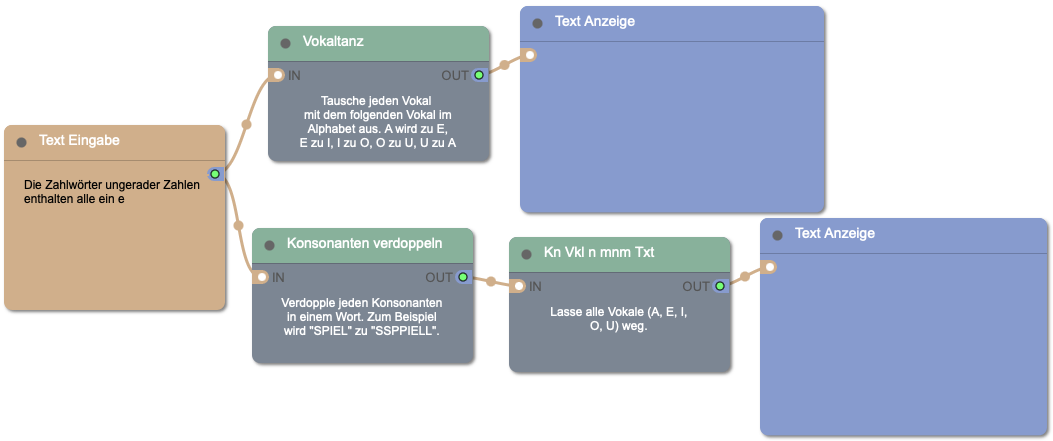
\includegraphics[width=\textwidth]{Bilder/Wortmaschinen_A1_config.png}

\section{ Maschinen verketten}
Zwei Maschinen kannst du in unterschiedlicher Reihenfolge verbinden. Spielt die Reihenfolge eine Rolle für das Ergebnis? Probiere es aus und begründe deine Antwort.\par
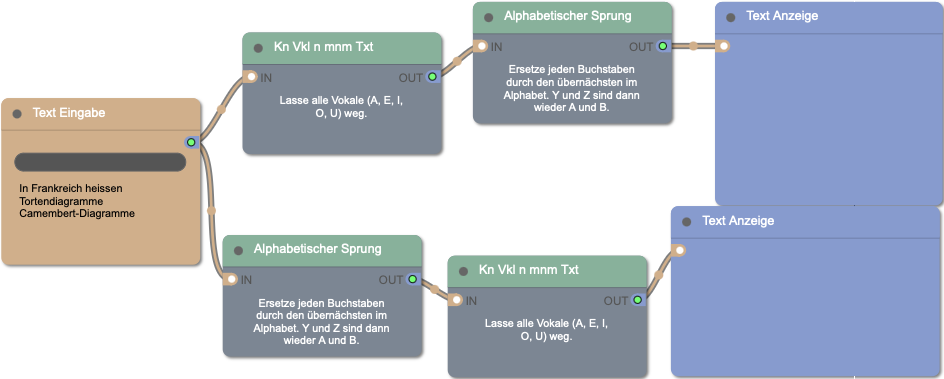
\includegraphics[width=\textwidth]{Bilder/Wortmaschinen_A2_config.png}
\handwritinglines{3}\\
Ist das immer so? Findest du zwei, bei denen die Reihenfolge egal ist? Gib die gefundenen Maschinen an, notiere den Ergebnis-Text und erkläre, was hier anders ist. Eine Übersicht über alle Wortmaschinen findest du am Ende dieses Arbeitsmaterials.\par
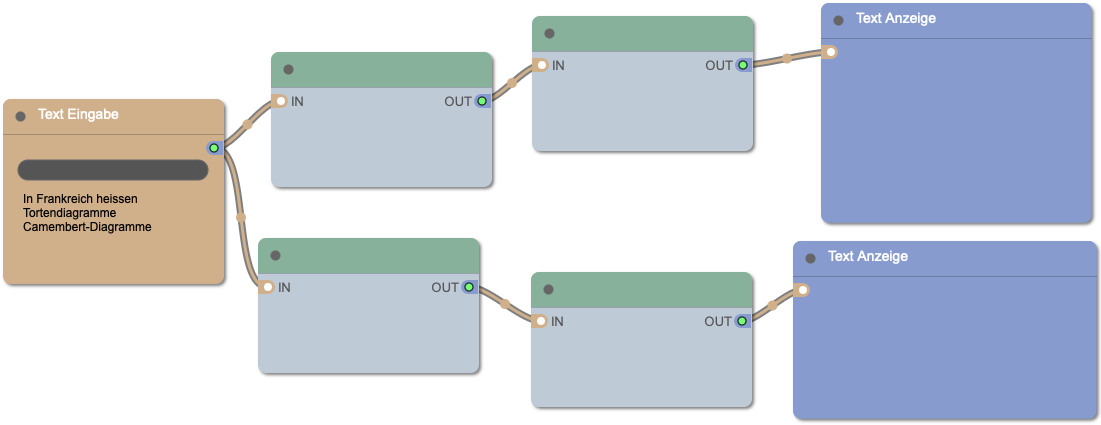
\includegraphics[width=\textwidth]{Bilder/Wortmaschinen_A2b_config.png}

\section{Welche Maschine war es?}
Hier sind zwei Nachrichten verschlüsselt worden. Einmal mit einer Maschine und einmal mit zwei Maschinen hintereinander.\par
Überlege erst was am Text verändert wurde und welche Maschinen es gewesen sein könnten. Probiere es aus und schreib den Namen der richtigen Maschine in das entsprechende Feld.\par
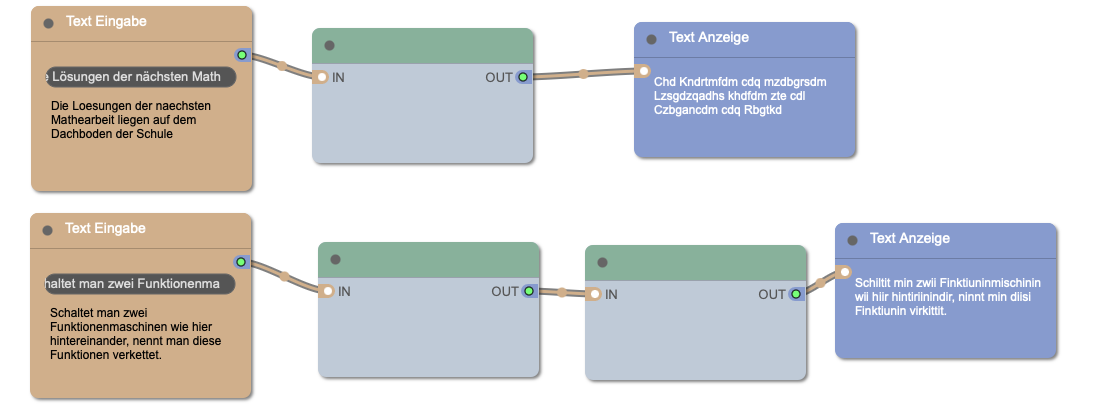
\includegraphics[width=\textwidth]{Bilder/Wortmaschinen_A3_config.png}


\section{Entschlüsseln einer Nachricht}
Mit der Alphabet-Countdown-Maschine wurde eine Nachricht verschlüsselt. Entwickle eine Maschine, um die Nachricht wieder zu entschlüsseln. Gib ihr einen Namen und beschreibe ihre Funktionsweise auf der Karte.\par
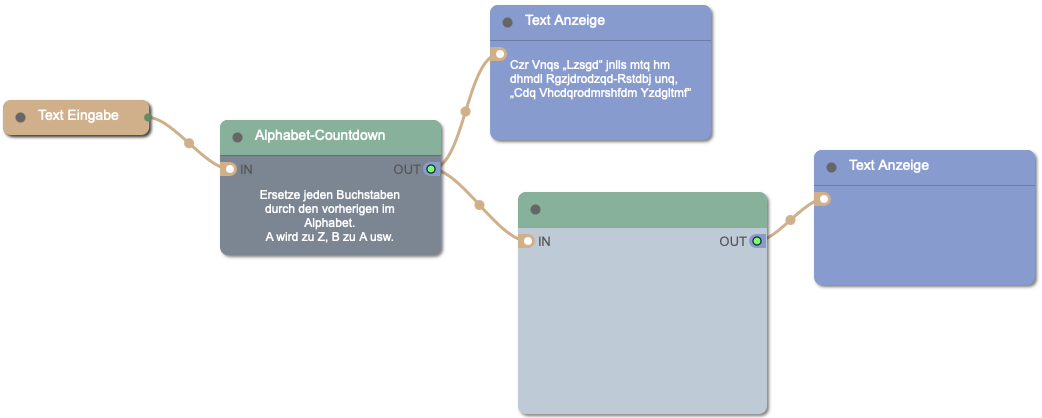
\includegraphics[width=\textwidth]{Bilder/Wortmaschinen_A4_config.png}\\
Genau die richtige Maschine zum Entschlüsseln der Botschaft scheint es in MATH-NODES nicht zu geben. Kannst du Sie aus anderen Maschinen zusammenbauen? Wie lautet die Botschaft? \\
\handwritinglines{2}

\section{ Umkehrbar oder nicht?}
Kannst du dir zu jeder Maschine eine Maschine ausdenken, die die damit verschlüsselte Nachricht wieder entschlüsselt?\par
Finde in MATH-NODES mindestens ein Beispiel, bei dem es nicht geht und begründe warum.\\
\handwritinglines{4}
\subsection{Bonusaufgabe:}
Mit welcher Maschine wurde hier verschlüsselt und wie kannst du das Rückgängig machen?\par
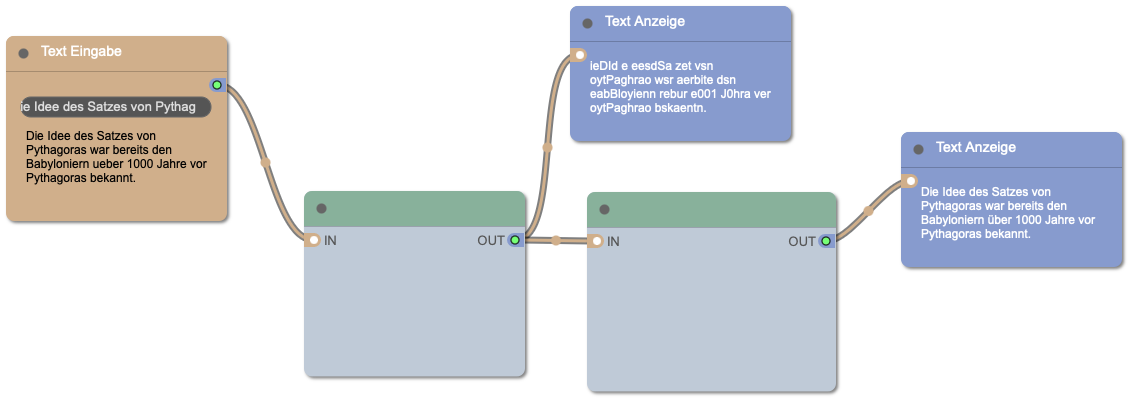
\includegraphics[width=\textwidth]{Bilder/Wortmaschinen_A5_config.png}
\handwritinglines{2}
\section{Umkehrfunktionen}
Überlege welche der Wortmaschinen Umkehrfunktionen zueinander sind. Gib Sie an, begründe deine Entscheidung und prüfe an einem Beispiel. Eine Übersicht über alle Maschinen findest du am Ende des Kapitels.\par
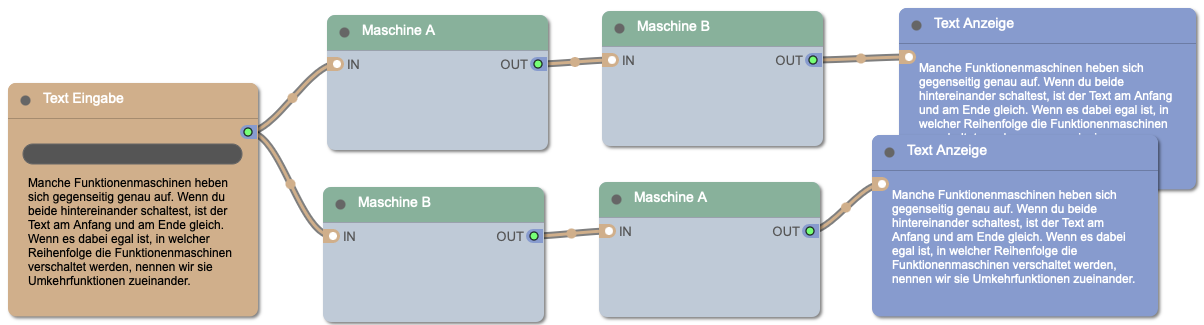
\includegraphics[width=\textwidth]{Bilder/Wortmaschinen_A6_config.png}
\handwritinglines{7}
\section{Geheime Nachrichten senden}
Überleg dir eine Nachrichten für die Person neben dir und schreib sie auf. Wähle bis zu drei Wortmaschinen zum Verschlüsseln aus, gib sie an und verschlüssele deine Nachricht damit. Achte bei der Auswahl deiner Wortmaschinen darauf, dass die Nachricht auch wieder entschlüsselbar ist.\par
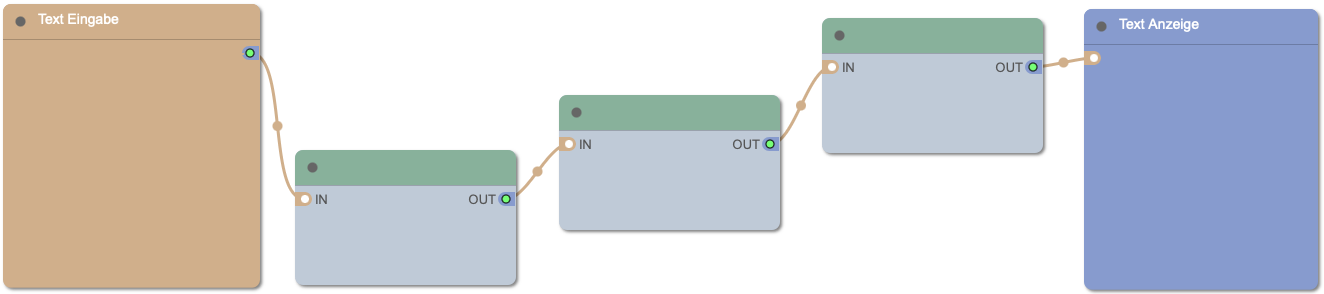
\includegraphics[width=\textwidth]{Bilder/Wortmaschinen_A7_config.png} 
\section{Geheime Nachrichten empfangen}
Tauscht eure verschlüsselten Nachrichten aus und probiert sie wieder zu entschlüsseln. Notiere deine empfangene Nachricht und deine Lösung.\par
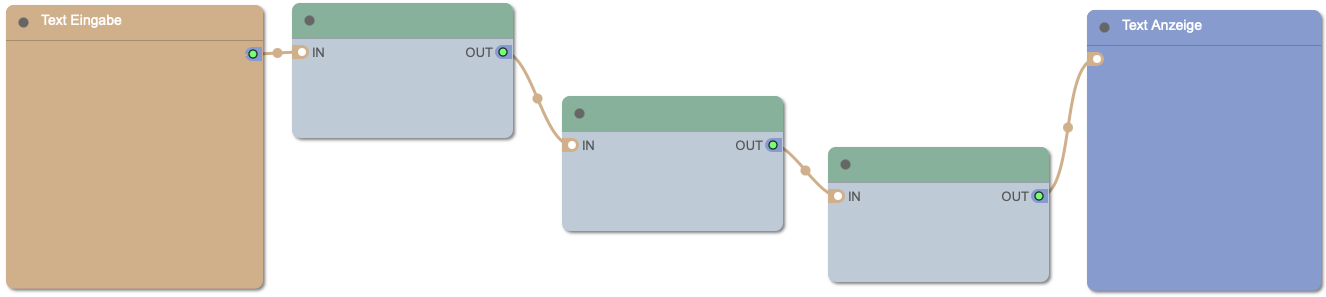
\includegraphics[width=\textwidth]{Bilder/Wortmaschinen_A8_config.png} 
\section*{Übersicht über alle Wortmaschinen}
\addcontentsline{toc}{section}{Übersicht über alle Wortmaschinen} % Add the chapter title to the table of contents 
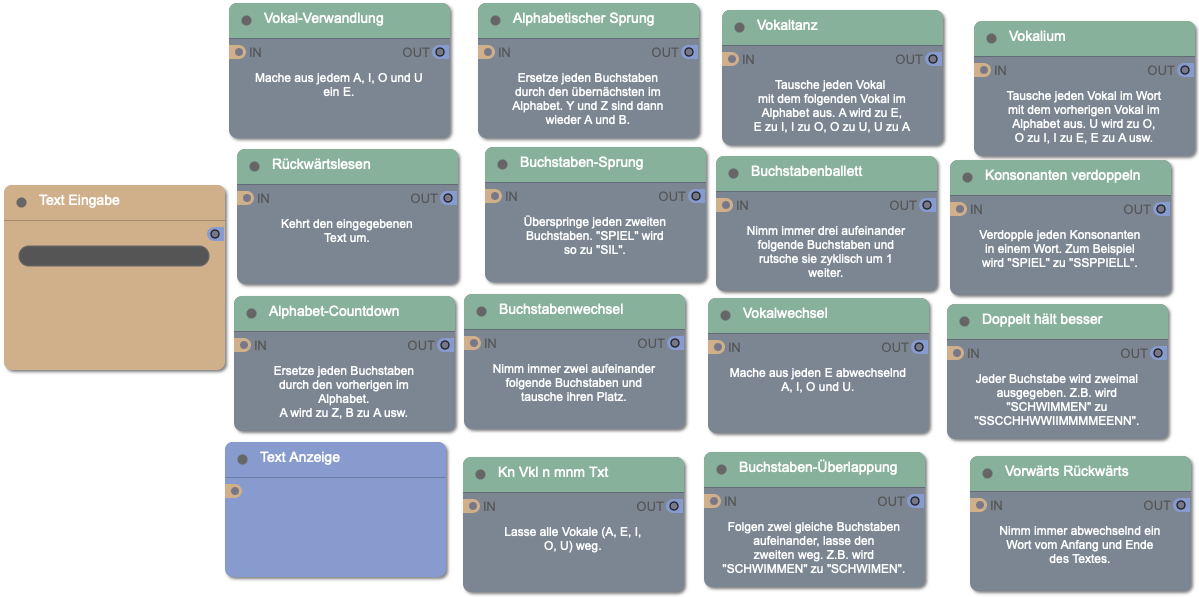
\includegraphics[width=\textwidth]{Bilder/Uebersicht_Wortmaschinen.png}
\chapterstartpage{Funktionsmaschinen}{MATHEMATISCHE FUNKTIONEN VERKNÜPFEN UND VERKETTEN LERNEN}{customlightpurple}


\newpage


\newpage


\end{document}